
          %-------------------------------%
\chapter{~~Finite elements and integrators}\label{\numb section 6}
          %-------------------------------%


Finite elments are still incipient in \maniFEM.
Paragraph \ref{\numb section 6.\numb parag 1} discusses the concept of finite element
and paragraphs \ref{\numb section 6.\numb parag 2} -- \ref{\numb section 6.\numb parag 4}
give examples of rudimentary use.
There is a lot of ongoing work on this subject.


          %---------------%
\section{~~Finite elements}\label{\numb section 6.\numb parag 1}
          %---------------%

The notion of a finite element is quite complex.
The purpose of a {\small\tt \verm{FiniteElement}} is to build a list of functions, say, $ \psi $,
defined on our mesh.
The linear span of these functions will be a discretized Hilbert space.
It is the {\small\tt \verm{FiniteElement}}'s job to replace, in the variational formulation,
the unknown function by one $ \psi $, the test function by another $ \psi $ and,
by evaluating the integrals, obtain the coefficients of a system of linear equations.
Some external solver will then solve the system, and it is the job of the finite element
to transform back the vector produced by the solver into a function defined on our mesh.

Computing each integral is a somewhat separate process; it's the job of an
{\small\tt \verm{Integrator}}
which could be a Gauss quadrature or some other procedure like symbolic integration.
When a Gauss quadrature is used, the separation between a {\small\tt \verm{FiniteElement}}'s job
and the {\small\tt \verm{Itegrator}}'s job is not very sharp because often the Gauss quadrature is
perfomed not on the physical cell but rather on a master element which is built and
handled by the {\small\tt \verm{FiniteElement}}.
The authors of {\maniFEM} have tried to separate these two concepts
as much as possible, especially because some users may want to use a {\small\tt \verm{FiniteElement}}
with no master element, or an {\small\tt \verm{Integrator}} acting directly on the physical cell.

Thus, there is a base class {\small\tt \verm{FiniteElement}} and a derived class
{\small\tt \verm{FiniteElement}::withMaster} which keeps, as an extra attribute, the map transforming
the master element to the current physical cell.
This map depends of course on the geometry of the cell and thus it must be computed from
scratch each time we begin integrating on a new cell.
We say that the {\small\tt \verm{FiniteElement}} is docked on a new {\small\tt \verm{Cell}};
the method {\small\tt dock\_\,on} performs this operation.
This method is element-specific, each type of finite element having its own class.

For instance, the class {\small\tt \verm{FiniteElement}::Lagrange\_\,Q1} is a class derived from
{\small\tt \verm{FiniteElement}:: ::withMaster}.
It will only {\small\tt dock\_\,on} quadrilaterals (two-dimensional {\small\tt \verm{Cell}}s
with four sides).
% Recall that in {\maniFEM} the vertices do not have necessarily any number attached.
% When we create a {\small\tt \verm{FiniteElement}::Lagrange\_\,Q1} object, it will enumerate vertices
% of the mesh if a mesh exists already, and it will prepare the ground for vertices created
% in the future to be enumerated, too.
% This enumeration is useful to identify a vector of real numbers with the values
% (at each vertex) of a function defined on the mesh.
When docking on a cell, the {\small\tt \verm{FiniteElement}::Lagrange\_\,Q1} object will build four
``shape functions'' and a transformation map (a diffeomorphism between a master element
occuppying the square $ [-1, 1]^2 $ and the current cell).
It will also build the jacobian of this transformation map.
The four shape functions can be accessed through the method {\small\tt basis\_\,function},
as shown in paragraph \ref{\numb section 6.\numb parag 2}.

It should be stressed that the approach presented in this section is rather low-level.
We are working hard to make {\maniFEM} understand statements describing variational
formulations given as {\tt C++} objects.
When this part of the code is done, the programming style will become much more elegant
and compact.

Note also that these examples make use of the {\small\tt Eigen} library.


          %------------------------------------------------%
\section{~~Laplace operator, Dirichlet boundary conditions}\label{\numb section 6.\numb parag 2}
          %------------------------------------------------%
\vskip 1mm

Let's look at an example about the Laplace operator with non-homogeneous Dirichlet
boundary conditions.
\vskip 1mm

\begin{Verbatim}[commandchars=\\\{\},formatcom=\small\tt,frame=single,
   label=parag-\ref{\numb section 6.\numb parag 2}.cpp,rulecolor=\color{coment},
   baselinestretch=0.94,framesep=2mm                                            ]
   \verm{Manifold} \azul{RR2} ( \textcolor{tag}{tag}::Euclid, \textcolor{tag}{tag}::of_dim, 2 );
   \verm{Function} \azul{xy} = RR2 .build_coordinate_system ( \textcolor{tag}{tag}::Lagrange, \textcolor{tag}{tag}::of_degree, 1 );
   \verm{Function} \azul{x} = xy [0], \azul{y} = xy [1];

   \cinza{// declare the type of finite element}
   \verm{FiniteElement} \azul{fe}
      ( \textcolor{tag}{tag}::with_master, \textcolor{tag}{tag}::quadrangle, \textcolor{tag}{tag}::Lagrange, \textcolor{tag}{tag}::of_degree, 1 );
   \verm{Integrator} \azul{integ} = fe .set_integrator ( \textcolor{tag}{tag}::Gauss, \textcolor{tag}{tag}::quad_4 );

   \cinza{// build a 10x12 mesh on a square domain}
   \verm{Cell} \azul{A} ( \textcolor{tag}{tag}::vertex );  x (A) = 0.;   y (A) = 0.;
   \verm{Cell} \azul{B} ( \textcolor{tag}{tag}::vertex );  x (B) = 1.;   y (B) = 0.;
   \verm{Cell} \azul{C} ( \textcolor{tag}{tag}::vertex );  x (C) = 1.;   y (C) = 1.;
   \verm{Cell} \azul{D} ( \textcolor{tag}{tag}::vertex );  x (D) = 0.;   y (D) = 1.;
   \verm{Mesh} \azul{AB} ( \textcolor{tag}{tag}::segment, A .reverse(), B, \textcolor{tag}{tag}::divided_in, 10 );
   \verm{Mesh} \azul{BC} ( \textcolor{tag}{tag}::segment, B .reverse(), C, \textcolor{tag}{tag}::divided_in, 12 );
   \verm{Mesh} \azul{CD} ( \textcolor{tag}{tag}::segment, C .reverse(), D, \textcolor{tag}{tag}::divided_in, 10 );
   \verm{Mesh} \azul{DA} ( \textcolor{tag}{tag}::segment, D .reverse(), A, \textcolor{tag}{tag}::divided_in, 12 );
   \verm{Mesh} \azul{ABCD} ( \textcolor{tag}{tag}::rectangle, AB, BC, CD, DA );
\end{Verbatim}
\vskip 1mm

A finite element can handle by itself the numbering of vertices, as shown in paragraph
\ref{\numb section 6.\numb parag 4}.
For now, we prefer the conceptually simpler approach of building by hand a {\small\tt map}
for numbering vertices.
\vskip 1mm

\begin{Verbatim}[commandchars=\\\{\},formatcom=\small\tt,frame=single,
   label=parag-\ref{\numb section 6.\numb parag 2}.cpp,rulecolor=\color{coment},
   baselinestretch=0.94,framesep=2mm                                            ]
   std::map < Cell, size_t > \azul{numbering};
   \verm{Mesh}::Iterator \azul{it} = ABCD .iterator ( \textcolor{tag}{tag}::over_vertices );
   size_t \azul{counter} = 0;
   for ( it .reset() ; it .in_range(); it++ )
   \{  \verm{Cell} \azul{V} = *it;  numbering [V] = counter;  ++counter;  \}
\end{Verbatim}
\vskip 1mm

The matrix of the linear system and the vector holding the free coefficients
are declared as objects of the {\small\tt Eigen} library.

\begin{Verbatim}[commandchars=\\\{\},formatcom=\small\tt,frame=single,
   label=parag-\ref{\numb section 6.\numb parag 2}.cpp,rulecolor=\color{coment},
   baselinestretch=0.94,framesep=2mm                                            ]
   size_t \azul{size_matrix} = ABCD .number_of ( \textcolor{tag}{tag}::vertices );
   assert ( size_matrix == numbering .size() );
   Eigen::SparseMatrix < double > \azul{matrix_A} ( size_matrix, size_matrix );
   Eigen::VectorXd \azul{vector_b} ( size_matrix );  vector_b .setZero();
\end{Verbatim}
\vskip 1mm

We now run over all rectangular cells of {\small\tt ABCD}, dock the finite element
on the current cell,
compute integrals of the form $ \displaystyle \int\!\!\!\int {\partial \psi_i \over
\partial x_\alpha} {\partial \psi_j \over \partial x_\beta} dx $ and add the obtained
values to the global matrix:
\vskip 1mm

\begin{Verbatim}[commandchars=\\\{\},formatcom=\small\tt,frame=single,
   label=parag-\ref{\numb section 6.\numb parag 2}.cpp,rulecolor=\color{coment},
   baselinestretch=0.94,framesep=2mm                                            ]
   // run over all square cells composing ABCD
   \verm{Mesh}::Iterator \azul{it} = ABCD .iterator ( \textcolor{tag}{tag}::over_cells_of_dim, 2 );
   for ( it .reset(); it .in_range(); it++ )
   \{  \verm{Cell} \azul{small_square} = *it;
      fe .dock_on ( small_square );
      // run twice over the four vertices of 'small_square'
      \verm{Mesh}::Iterator \azul{it1} = small_square .boundary() .iterator ( \textcolor{tag}{tag}::over_vertices );
      \verm{Mesh}::Iterator \azul{it2} = small_square .boundary() .iterator ( \textcolor{tag}{tag}::over_vertices );
      for ( it1 .reset(); it1 .in_range(); it1++ )
      for ( it2 .reset(); it2 .in_range(); it2++ )
      \{  \verm{Cell} \azul{V} = *it1, \azul{W} = *it2;
         \cinza{// V may be the same as W, no problem about that}
         \verm{Function} \azul{psiV} = fe.basis_function(V),
                  \azul{psiW} = fe .basis_function (W),
                  \azul{d_psiV_dx} = psiV .deriv (x),
                  \azul{d_psiV_dy} = psiV .deriv (y),
                  \azul{d_psiW_dx} = psiW .deriv (x),
                  \azul{d_psiW_dy} = psiW .deriv (y);
                  
         \cinza{// 'fe' is already docked on 'small_square'}
         \cinza{// so this will be the domain of integration}
         matrix_A .coeffRef ( numbering[V], numbering[W] ) +=
            fe .integrate ( d_psiV_dx * d_psiW_dx + d_psiV_dy * d_psiW_dy );    \}  \}
\end{Verbatim}

In the above, {\small\tt coeffRef} is the method used by {\small\tt Eigen} to access elements of
a sparse matrix.

We impose Dirichlet boundary conditions $ u(x,y) = xy $ (this way, we know beforehand
the exact solution will be $ u(x,y) = xy $).
We use a function {\small\tt impose\_\,value\_\,of\_\,unknown} which changes the {\small\tt matrix\_\,A}
and the {\small\tt vector\_\,b} in order to impose the Dirichlet condition {\small\tt u(i) = 
some\_\,value}.
See the source code in file {\small\tt main-\ref{\numb section 6.\numb parag 2}.cpp}
in the distribution tree for the definition of the {\small\tt impose\_\,value\_\,of\_\,unknown}
function.

\begin{Verbatim}[commandchars=\\\{\},formatcom=\small\tt,frame=single,
   label=parag-\ref{\numb section 6.\numb parag 2}.cpp,rulecolor=\color{coment},
   baselinestretch=0.94,framesep=2mm                                            ]
   \verm{Mesh}::Iterator \azul{it} = BC .iterator ( \textcolor{tag}{tag}::over_vertices );
   for ( it .reset(); it .in_range(); it++ )
   \{   \verm{Cell} \azul{P} = *it;
       size_t \azul{i} = numbering [P];
       impose_value_of_unknown ( matrix_A, vector_b, i, y(P) );  \}
\end{Verbatim}

We then use {\small\tt Eigen} to solve the system of linear equations :

\begin{Verbatim}[commandchars=\\\{\},formatcom=\small\tt,frame=single,
   label=parag-\ref{\numb section 6.\numb parag 2}.cpp,rulecolor=\color{coment},
   baselinestretch=0.94,framesep=2mm                                            ]
   Eigen::ConjugateGradient < Eigen::SparseMatrix <double>,
                              Eigen::Lower | Eigen::Upper  > \azul{cg};
   cg .compute ( matrix_A );
   Eigen::VectorXd \azul{u} = cg .solve ( vector_b );
\end{Verbatim}

And obtain the expected solution, shown in figure \ref{\numb section 6.\numb fig 1}.

\begin{figure} \centering
  \psfrag{A}{\small\tt\textcolor{textindraw}{A}}
  \psfrag{B}{\small\tt\textcolor{textindraw}{B}}
  \psfrag{C}{\small\tt\textcolor{textindraw}{C}}
  \psfrag{D}{\small\tt\textcolor{textindraw}{D}}
  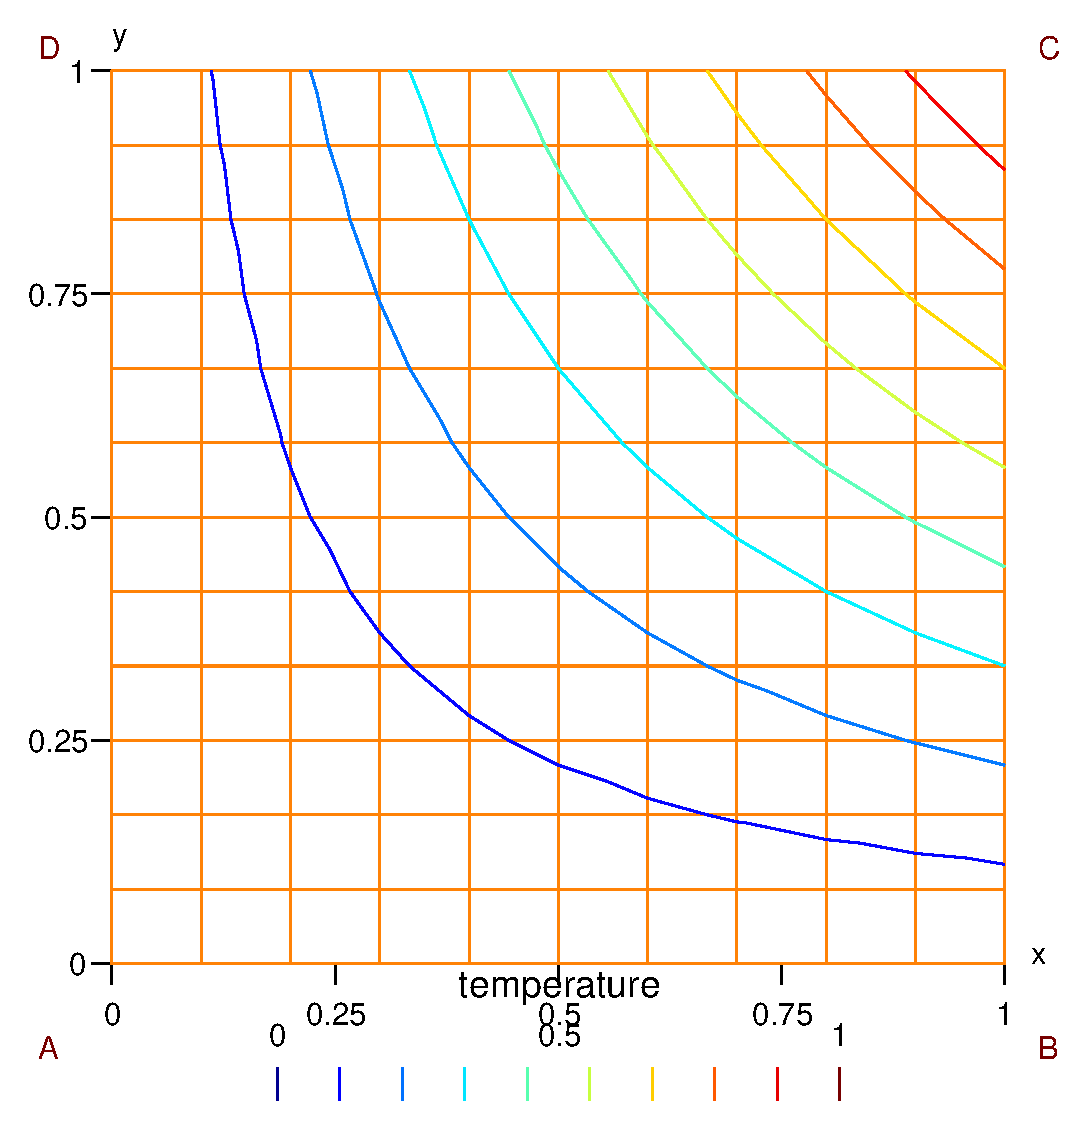
\includegraphics[width=60mm]{square-Dirichlet}
  \caption{Level lines of $u$}
  \label{\numb section 6.\numb fig 1}
\end{figure}

We stress again that this example shows a rather rudimentary way of using finite elements in
\maniFEM.
We are working hard to reach a more elegant, compact and high-level style.
The user should have the possibility to declare the partial differential equation
through a compact declaration of the corresponding variational formulation.

Another limitation of {\maniFEM} is that, at present, finite element computations
are rather slow.
This is so because each docking operation implies a lot of symbolic calculations;
the same happens when we differentiate and then integrate functions.
There are three ways of circumventing this limitation.
The first one is : if your mesh is made of identical finite elements
(like the example in the present paragraph), you can compute the elementary matrix
just once and then assembly the global matrix from it.
It will surely be much faster.
A second way to speed up the code is to add the option {\small\tt -dNDEBUG} to the compilation
command in your {\small\tt Makefile} (see also paragraph \ref{\numb section 11.\numb parag 15}).

The third (and soundest) solution is a deep optimization of the {\maniFEM} library.
A new type of finite elements (or, rather, integrators) is object of on-going work.
These integrators perform a few symbolic calculations just once,
typically right after they are declared.
Only raw arithmetic operations are performed when the user actually requests the values
of integrals in order to assembly the matrix.


          %---------------------------%
\section{~~Neumann boundary conditions}\label{\numb section 6.\numb parag 3}
          %---------------------------%

Implementing zero Neumann boundary conditions does not imply any programming effort
(we don't have to do anything).
However, for imposing non-zero Neumann boundary conditions we need to compute one-dimensional
integrals.
We do this by declaring a 1D finite element which we then dock on each segment of the
part of the boundary where we need to integrate.

\begin{Verbatim}[commandchars=\\\{\},formatcom=\small\tt,frame=single,
   label=parag-\ref{\numb section 6.\numb parag 3}.cpp,rulecolor=\color{coment},
   baselinestretch=0.94,framesep=2mm                                            ]
   \verm{FiniteElement} \azul{fe_bdry} ( \textcolor{tag}{tag}::with_master, \textcolor{tag}{tag}::segment,
                           \textcolor{tag}{tag}::Lagrange, \textcolor{tag}{tag}::of_degree, 1 );
   \verm{Integrator} \azul{integ_bdry} = fe_bdry .set_integrator ( \textcolor{tag}{tag}::Gauss, \textcolor{tag}{tag}::seg_3 );

   \cinza{// ... assemble the matrix ...}

   \verm{Function} \azul{heat_source} = x+y;
   \cinza{// impose Neumann boundary conditions du/dn = heat_source :}
   \verm{Mesh}::Iterator \azul{it} = DA .iterator ( \textcolor{tag}{tag}::over_segments );
   for ( it .reset(); it .in_range(); it++ )
   \{  \verm{Cell} \azul{seg} = *it;
      fe_bdry .dock_on ( seg );
      \verm{Cell} \azul{V} = seg .base() .reverse();
      assert ( V .is_positive() );
      size_t \azul{i} = numbering [V];
      \verm{Function} \azul{psiV} = fe_bdry .basis_function(V);
      vector_b[i] += fe_bdry.integrate ( heat_source * psiV );
      \verm{Cell} \azul{W} = seg.tip();
      assert ( W .is_positive() );
      size_t \azul{j} = numbering [W];
      \verm{Function} \azul{psiW} = fe_bdry .basis_function(W);
      vector_b [j] += fe_bdry .integrate ( heat_source * psiW );  \}
\end{Verbatim}

One may object that there is no need for a 1D finite element, a 1D integrator should be enough.
We agree; the user should have the possibility to attach a 1D integrator to a 2D finite element.
This is object of on-going work.


          %------------------------------%
\section{~~Automatic numberig of vertices}\label{\numb section 6.\numb parag 4}
          %------------------------------%

In previous examples we have built a {\small\tt map} for handling numbering of vertices.
In this paragraph we show how to use instead the automatic numbering associated to the
finite element itself.
After declaring a finite element of type Lagrange with
{\small\tt\textcolor{tag}{tag}::enumerate\_\,cells},
the process of creating new cells (vertices, in this specfic case) will be different.
A new function will be added to the list of functions
{\small\tt\verm{Cell}::init\_\,pos\_\,cell[0]},
invoked by {\small\tt\verm{Cell}::Core} constructors
(see paragraph \ref{\numb section 11.\numb parag 10}).
Space will be reserved for a {\small\tt size\_\,t} value for each vertex, and
this value can be used for numbering vertices.

\begin{Verbatim}[commandchars=\\\{\},formatcom=\small\tt,frame=single,
   label=parag-\ref{\numb section 6.\numb parag 4}.cpp,rulecolor=\color{coment},
   baselinestretch=0.94,framesep=2mm                                            ]
   \verm{FiniteElement} \azul{fe} ( \textcolor{tag}{tag}::with_master, \textcolor{tag}{tag}::quadrangle,
                      \textcolor{tag}{tag}::Lagrange, \textcolor{tag}{tag}::of_degree, 1, \textcolor{tag}{tag}::enumerate_cells );
   \verm{Cell}::Numbering & \azul{numbering} = fe .numbering ( \textcolor{tag}{tag}::vertices );
\end{Verbatim}

In this approach, the access to the index of a given vertex is very fast (constant time)
because the index is stored within the {\small\tt\verm{Cell}::Core}, so no search is needed.
In contrast, when using a {\small\tt map} as shown in paragraph
\ref{\numb section 6.\numb parag 2}, a search is necessary through all vertices of the mesh.
Due to the implementation of the {\small\tt map} class in {\tt STL}, this search takes
logarithmic time.
The only advantage of the approach described in paragraph \ref{\numb section 6.\numb parag 2}
is that the user has full contol of the numbering (see below).

Using the numbering associated to the finite element itself has the following disadvantage.
This automatic numbering process does not distinguish between vertices created at the user's
request and other vertices used internally by different components of {\maniFEM};
these vertices are invisible to the user.
As a consequence, the numbering will not be contiguous.
Lines of the global matrix corresponding to ``missing'' vertices are not significant in any way.
Columns corresponding to missing vertices are not significant either (because they will only
have zero entries).
However, the solver of the linear system will complain that the matrix is singular.
To circumvent this problem, we insert a non-zero value in the diagonal of the global matrix
at places corresponding to ``missing'' vertices.
This is equivalent to imposing a Dirichlet boundary condition on those vertices.
Since we have no way of running over the missing vertices, we first fill the entire
diagonal with ones, then erase them for existing vertices.

\begin{Verbatim}[commandchars=\\\{\},formatcom=\small\tt,frame=single,
   label=parag-\ref{\numb section 6.\numb parag 4}.cpp,rulecolor=\color{coment},
   baselinestretch=0.94,framesep=2mm                                            ]
   for ( size_t \azul{i} = 0; i < size_matrix; i++ )
      matrix_A .insert ( i, i ) = 1.;
   \verm{Mesh}::Iterator \azul{it} = ABCD .iterator ( \textcolor{tag}{tag}::over_vertices );
   for ( it .reset(); it .in_range(); it++ )
   \{  \verm{Cell} \azul{P} = *it;
      size_t \azul{i} = numbering ( P );
      matrix_A .coeffRef ( i, i ) = 0.;  \}
\end{Verbatim}

The rest of the code is identical to paragraph \ref{\numb section 6.\numb parag 2}.

A different way around can be used, which allows the use of a {\small\tt matrix\_\,A}
with the correct dimension (equal to the number of vertices in the mesh {\small\tt ABCD}).
We simply assign the desired value to the numbering of each vertex :

\begin{Verbatim}[commandchars=\\\{\},formatcom=\small\tt,frame=single,
   rulecolor=\color{coment},baselinestretch=0.94,framesep=2mm          ]
   \verm{Mesh}::Iterator \azul{it} = ABCD .iterator ( \textcolor{tag}{tag}::over_vertices );
   size_t \azul{counter} = 0;
   for ( it .reset(); it .in_range(); it++ )
   \{  \verm{Cell} \azul{P} = *it;
      numbering ( P ) = counter++;  \}
\end{Verbatim}

This solution keeps the advantage of constant accesss time to the number of a vertex.
However, the information from {\small\tt numbering.size()} will be misleading
(it still takes into account the ``hidden'' vertices).
You should use instead {\small\tt ABCD.number\_\,of} {\small\tt} {\small\tt (}
{\small\tt \textcolor{tag}{tag}::vertices )}; this is the dimension you should use
when declaring your global matrix.

Note that both numbering methods (presented in paragraphs \ref{\numb section 6.\numb parag 2}
and \ref{\numb section 6.\numb parag 4}) allow for retrieving
an index of a given vertex but not the other way around.
If you need to retrieve a vertex from its index you should probably use 
a vector of {\small\tt\verm{Cell}}s.

For the example in paragraph \ref{\numb section 6.\numb parag 3}, you should add the
{\small\tt\textcolor{tag}{tag}::enumerate\_\,cells} when declaring {\small\tt fe} and not when
declaring {\small\tt fe\_\,bdry} -- you don't want two independent mechanisms for numbering
vertices, do you ?
